\chapter{2020年\textsf{HDU} 概率论与数理统计期中试卷\textsf A}

\begin{minipage}{0.32\textwidth}
    \textbf{开课学院}：理学院
      
    \textbf{课程编码}：A0714040
\end{minipage}
\hfill
\begin{minipage}{0.32\textwidth}
    \textbf{解析制作}：\textsc{Ljl, Zzr, Zwx, Xxy}

    \textbf{\,\hologo{TeX}~排版}：\textsc{Mingyu Hsia}
\end{minipage}
\hfill
\begin{minipage}{0.15\textwidth}
    \centering
    \begin{tikzpicture}
        \node [inner sep=0] at (0,0) {
            \qrcode[height=3em,level=M]{https://qm.qq.com/q/OlkSiy9W04}};
        \fill [color=white,rounded corners] (-.5em,-.5em) rectangle (.5em,.5em);
        \node [inner sep=0] at (0,0) {\color{MidnightBlue}\scriptsize\faIcon{qq}};
    \end{tikzpicture}

    \scriptsize\href{https://qm.qq.com/q/OlkSiy9W04}{\itshape 未央数学营}
\end{minipage}
\hfill
\begin{minipage}{0.15\textwidth}
    \centering
    \begin{tikzpicture}
        \node [inner sep=0] at (0,0) {
            \qrcode[height=3em,level=M]{http://weixin.qq.com/r/DBIABcHEqgnWKIVmb0eI}};
        \fill [color=white,rounded corners] (-.5em,-.5em) rectangle (.5em,.5em);
        \node [inner sep=0] at (0,0) {\color{DarkGreen}\scriptsize\faIcon{weixin}};
    \end{tikzpicture}

    \scriptsize\href{http://weixin.qq.com/r/DBIABcHEqgnWKIVmb0eI}{\itshape 未央学社}
\end{minipage}

\section{选择题（每题3分，共15分）}

\begin{problem}
    设随机事件$A$、$B$满足$P(B|A)=1$，则
    \begin{tasks}(4)
        \task $P(A)=P(B)$
        \task $P(AB)=0$
        \task $B\subset A$
        \task[\true] $A\subset B$
    \end{tasks}
\end{problem}
\begin{solution}
    由于$P(B|A)=P(AB)/P(A)=1$，所以$P(AB)=P(A)\neq 0$，$A\subset B$.
\end{solution}

\begin{problem}
    设随机变量$X$服从正态分布$N(\mu,\sigma^2)$，则随$\sigma$的增大，$P\ab\{\abs{\frac{x-\mu}{\sigma}<1}\}$的概率
    \begin{tasks}(4)
        \task 单调递增
        \task 单调递减
        \task[\true] 保持不变
        \task 增减不定
    \end{tasks}
\end{problem}
\begin{solution}
    由于$(X-\mu)/\sigma$是标准化的过程，所以$(X-\mu)/\sigma\sim N(0,1)$. 令$Y=(X-\mu)/\sigma$，$Y\sim N(0,1)$，即$P\{\abs Y<1\}$，所以概率不变.
\end{solution}

\begin{problem}
    设$A$和$B$是任意两个概率不为零的互不相容（互斥）的随机事件，则下列结论中肯定正确的是
    \begin{tasks}(2)
        \task $P(\overline A~\overline B)\neq0$
        \task $P(\overline A~\overline B)=0$
        \task $P(AB)=P(A)P(B)$
        \task[\true] $P(A-B)=P(A)$
    \end{tasks}
\end{problem}
\solute2
\begin{solution}\leavevmode
    \begin{itemize}
        % \task 反例如图：\tikz[baseline=.375em]{
        %     \draw [thick] (0,0) rectangle (.5,.5) node [midway] {$A$};
        %     \draw [thick] (.5,0) rectangle (1,.5) node [midway] {$B$};}. 所以A选项错误.
        % \task 反例如图：\tikz[baseline=.375em]{
        %     \filldraw [pattern=north east lines,pattern color=DarkGreen,even odd rule] (0,0) rectangle (1,.5) (.25,.25) circle (.2) node {$A$} (1,.5) (.75,.25) circle (.2) node {$B$};}. 所以B选项错误.
        \item 考虑A与B的并集是否是全集，所以A选项错误，B选项同理.
        \item 由于$P(AB)=0$，$P(A)$、$P(B)\neq0$，所以C选项错误.
        \item 由于$A$和$B$互斥，所以$P(A-B)=P(A)$，D选项正确.
    \end{itemize}
\end{solution}

\begin{problem}
    设$X\sim U(0,1)$，$Y\sim U(0,1)$，且$X$与$Y$相互独立，则二维随机变量$(X,Y)$的密度函数为
    \begin{tasks}(2)
        \task $f(x)=
            \begin{cases}
                x, & x\in(0,1)\\
                0, & \text{else}
            \end{cases}$
        \task $f(x)=
            \begin{cases}
                x, & x\in(0,1),\ y\in(0,1)\\
                0, & \text{else}
            \end{cases}$
        \task $f(x)=
            \begin{cases}
                y, & y\in(0,1)\\
                0, & \text{else}
            \end{cases}$
        \task[\true] $f(x)=
            \begin{cases}
                xy, & x\in(0,1),\ y\in(0,1)\\
                0, & \text{else}
            \end{cases}$
    \end{tasks}
\end{problem}
\solute1
\begin{solution}
    由于$X$、$Y$相互独立，所以联合概率密度仍服从均匀分布. 所以D选项正确.
\end{solution}

\begin{problem}
    已知连续型随机变量$X$的概率密度函数为$f(x)$是偶函数，$F(x)$是$X$的分布函数，则对于任意的实数$c$有$F(-c)$等于
    \begin{tasks}(4)
        \task[\true] $\displaystyle\frac12-\int_0^cf(x)\d x$
        \task $F(c)$
        \task $2F(c)-1$
        \task $\displaystyle1-\int_0^cf(x)\d x$
    \end{tasks}
\end{problem}
\solute3
\columnratio{.72}
\begin{paracol}{2}
\begin{solution}
    由于$f(x)$是偶函数，$f(c)=f(-c)$，所以有
    \[F(-c)=\frac12-\int_{-c}^0f(x)\d x=\frac12-\int_0^cf(x)\d x\]
    这里利用了$F(-c)=1-F(c)$，如右图所示. 所以A选项正确.
\switchcolumn
\vspace*{\fill}
\centering
\tikz{%
    \fill [pattern=north east lines,pattern color=DarkGreen] (-1.25,0) -- (-1.25,{exp(-1.25^2)}) -- (-.9,{exp(-.81)}) -- (-.9,0);
    \fill [pattern=north east lines,pattern color=DarkGreen] (1.25,0) -- (1.25,{exp(-1.25^2)}) -- (.9,{exp(-.81)}) -- (.9,0);
    \draw [thick,->] (-1.5,0) -- (1.5,0);
    \draw [thick,->] (0,-.5) -- (0,1.5);
    \draw [thick,densely dashed] (-.9,0) node [below] {$-c$} -- (-.9,{exp(-.81)});
    \draw [thick,densely dashed] (+.9,0) node [below] {$c$} -- (+.9,{exp(-.81)});
    \draw [very thick,teal,variable=\x,domain=-1.25:1.25,smooth,line cap=round] plot ({\x},{exp(-\x*\x)});
}
\vspace{\fill}
\end{solution}
\end{paracol}

\section{填空题}

\begin{problem}
    已知随机事件$A$与$B$相互独立，且$P(AB)=0.15$，$P(A)=0.3$，则$P(B)=$\ans{$0.5$}.
\end{problem}
\solute2
\begin{solution}
    $P(AB)=P(A)P(B)$，$P(B)=0.5$.
\end{solution}

\begin{problem}
    设$P(AB)=0.6$，则$P(\overline A\cup\overline B)=$\ans{$0.4$}.
\end{problem}
\solute1
\begin{solution}
    $1-P(\overline{\overline A\cup\overline B})=1-P(\overline{\overline A}\overline{\overline B})=1-P(AB)$. 所以$P(\overline A\cup\overline B)=1-P(AB)=0.4$.
\end{solution}

\begin{problem}
    设$X\sim N(5,\sigma^2)$，$P\{5<X<10\}=0.3$，则$P\{0<X<5\}=$\ans{$0.3$}.
\end{problem}
\solute2
\begin{solution}\leavevmode
    \begin{itemize}
        \item 由正态分布的性质知$X$的概率分布关于直线$x=\mu=10$对称.
        \item 所以$P\{0<X\leq 5\}=P\{5<X<10\}=0.3$.
    \end{itemize}
\end{solution}

\begin{problem}
    设随机变量$X$的密度函数为$f_X(x)=\begin{cases}
        2x, & 0<x<1\\
        0,  & \text{else}
    \end{cases}$. $Y$表示对$X$的三次独立重复观察中事件$\{X<1/3\}$出现的次数，则$P\{Y=2\}=$\ans{$8/243$}.
\end{problem}
\solute2
\begin{solution}
    $P(A)=\int_0^{1/3}2x\d x=1/9$，$Y\sim B(3,1/9)$，$P(Y=2)=C_3^2(1/9)^2\times8/9=8/243$.
\end{solution}

\begin{problem}
    设公共汽车从上午6时起，每15分钟发一趟车，已知某乘客在6:00到6:30任意时刻到达车站，则该乘客候车时间少于5分钟的概率为\ans{$1/3$}.
\end{problem}
\solute3
\begin{solution}
    $X\sim U(0,30)$，其概率密度函数为
    \[f(x)=\begin{cases}
        1/30, & 0<x<30\\0, & \text{else}
    \end{cases}\]
    乘客必须在6:10 -- 6:15或6:25 -- 6:30进站. 乘客候车时间少于5分钟的概率为
    \[P(10<x<15)+P(25<x<30)=\int_{10}^{15}\frac{1}{30}\d x+\int_{25}^{30}\frac{1}{30}\d x=\frac13\]
\end{solution}

\section{解答题}

\begin{problem}
    一批产品有12件，其中4件次品，8件正品. 现从中任取3件产品，试求取出的3件产品中有次品的概率.
\end{problem}
\solute3
\begin{solution}
    设$A=\{\text{取出的3件产品中有次品}\}$，则$P(A)=1-P(\overline A)=1-C_8^3/C_{12}^3=41/55$.
\end{solution}

\columnratio{.64}
\begin{paracol}{2}
\begin{problem}
    设随机变量$X$的分布律如右图所示. 求
    \begin{tasks}[label=\arabic*.](2)
        \task 常数$a$.
        \task $P\{-2\leq X<0\}$.
        \task $Y=X^2$的分布律.
    \end{tasks}
\end{problem}
\switchcolumn
\vspace*{\fill}
\begin{table}[htbp]
    \centering
    \begin{tabular}{cccccc}
        \toprule
        $X$ & $-2$ & $-1$ & $0$ & $1$ & $2$\\
        \midrule
        $P$ & $a$ & $3a$ & $1/8$ & $a$ & $2a$\\
        \bottomrule
    \end{tabular}
\end{table}
\vspace{\fill}
\end{paracol}
\solute5
\begin{paracol}{2}
\begin{solution}\leavevmode
    \begin{enumerate}
        \item $a+3a+1/8+a+2a=1$，$a=1/8$.
        \item $P\{-2\leq x<0\}=P\{x=-2\}+P\{x=-1\}=1/2$.
    \end{enumerate}
\switchcolumn
\vspace*{\fill}
\begin{figure}[htbp]
    \centering
    \begin{tabular}{cccc}
        \toprule
        $x^2$ & $0$ & $1$ & $4$\\
        \midrule
        $P$ & $1/8$ & $1/2$ & $3/8$\\
        \bottomrule
    \end{tabular}
\end{figure}
\end{solution}
\end{paracol}

\begin{problem}
    设随机变量的密度函数为
    \[f(x)=\begin{cases}
        4x^3, & 0<x<1\\
        0, & \text{else}
    \end{cases}\]
    \begin{multicols}{2}
        \begin{enumerate}
            \item 求$X$的分布函数$F(x)$.
            \item 求$Y=X^2$的密度函数$f_Y(y)$.
            \item 当$a$为何值时，$P\{x>a\}=P\{x<a\}$?
        \end{enumerate}
    \end{multicols}
\end{problem}
\solute3
\begin{solution}\leavevmode
    \begin{enumerate}
        \item 
        $F(x)=\begin{cases}
            \int_{-\infty}^xf(x)\d x=0, & x<0\\
            \int_{-\infty}^xf(x)\d x=\int_0^x4x^3\d x=x^4, & 0\leq x<1\\
            \int_0^14x^3\d x=1, & x\geq1
        \end{cases}$
        \item $F_Y(y)=P(Y\leq y)=P(x^2\leq y)$.
        \begin{itemize}
            \item $y<0$时，$F_Y(y)=0$.
            \item $y\geq0$时，$F_Y(y)=P(x^2\leq y)=F_X(\sqrt y)-F_X(-\sqrt y)=
            \begin{cases}
                y^2, & 0\leq y<1\\
                1, & y\geq1
            \end{cases}$
            \item 综上所述，$Y=X^2$的密度函数为
            $\begin{cases}
                2y, & 0\leq y<1\\
                0, & \text{else}
            \end{cases}$
        \end{itemize}
        \item $P(x>a)=1-P(x\leq a)=1-F(a)$，所以$P(x>a)=P(x<a)$，$F(a)=1/2$，$a=\sqrt[4]{1/2}$.
    \end{enumerate}
\end{solution}

\begin{paracol}{2}
\begin{problem}
    右图为二维随机变量$(X,Y)$的分布律. 求
    \begin{enumerate}
        \item $X$和$Y$的边缘分布律.
        \item $X/Y$的分布律.
        \item 当$Y=4$时，关于$X$的条件分布律.
    \end{enumerate}
\switchcolumn\vspace*{\fill}\centering
    \begin{tabular}{cccc}
        \toprule
        \diagbox YX & $2$ & $5$ & $8$\\
        \midrule
        $4$ & $0.15$ & $0.3$ & $0.35$\\
        \hline
        $8$ & $0.05$ & $0.12$ & $0.03$\\
        \bottomrule
    \end{tabular}\vspace*{\fill}
\end{problem}
\end{paracol}
\solute3
\begin{solution}$X$和$Y$的边缘分布律、$X/Y$的分布律分别为
    \begin{table}[htbp]
        \begin{minipage}{.24\textwidth}
            \centering
            \begin{tabular}{cccc}
                \toprule
                $X$ & $2$ & $5$ & $8$\\
                \midrule
                $P$ & $0.2$ & $0.42$ & $0.38$\\
                \bottomrule
            \end{tabular}
            \caption*{$X$的边缘分布律}
        \end{minipage}
        \hfill
        \begin{minipage}{.24\textwidth}
            \centering
            \begin{tabular}{cccc}
                \toprule
                $Y$ & $4$ & $8$\\
                \midrule
                $P$ & $0.8$ & $0.2$\\
                \bottomrule
            \end{tabular}
            \caption*{$Y$的边缘分布律}
        \end{minipage}
        \hfill
        \begin{minipage}{.48\textwidth}
            \centering
            \begin{tabular}{ccccccc}
                \toprule
                $X/Y$ & $1/4$ & $5/8$ & $1/2$ & $5/4$ & $1$ & $2$\\
                \midrule
                $P$ & $0.05$ & $0.12$ & $0.15$ & $0.3$ & $0.03$ & $0.35$\\
                \bottomrule
            \end{tabular}
            \caption*{$X/Y$的分布律}
        \end{minipage}
    \end{table}

    由于$P(x=x|y=4)=P(x=x,y=4)/P(y=4)$，所以有
    \begin{tasks}[label=\labelitemi](2)
        \task $P(x=2|y=4)=0.15/0.8=3/16$.
        \task $P(x=2|y=4)=0.15/0.8=3/16$.
        \task $P(x=5|y=4)=0.3/0.8=3/8$.
        \task $P(x=8|y=4)=0.35/0.8=7/16$.
    \end{tasks}
\end{solution}

\begin{problem}
    已知二维随机变量$(X,Y)$概率密度函数为
    \[f(x,y)=\frac{A}{(1+x^2)(1+y^2)},\ -\infty<x<+\infty,\ -\infty<y<+\infty\]
    \begin{enumerate}
        \item 求常数$A$.
        \item 求$P\{(X,Y)\in D\}$，其中$D$为直线$y=x$，$x=1$及$x$轴围成的三角形区域.
        \item 求$f_X(x)$，$f_Y(y)$.
        \item $X$，$Y$是否相互独立？说明理由. 已知$\displaystyle\int\frac1{1+x^2}\d x=\arctan x+C$.
    \end{enumerate}
\end{problem}
\solute3
\begin{solution}\leavevmode
    \begin{enumerate}
        \item $\displaystyle\int_{-\infty}^{+\infty}\int_{-\infty}^{+\infty}f(x,y)\d x\d y=1$，$A=1/\pi^2$.
        \item 
        $\displaystyle P\{(X,Y)\in D\}=\int_0^1\d x\int_0^x\frac{1}{\pi^2(1+x^2)(1+y^2)}\d y=\frac1{32}$.
        \item $X$和$Y$的边缘概率密度为
        \begin{itemize}
            \item $\displaystyle f_X(x)=\int_{-\infty}^{+\infty}f(x,y)\d y=\frac{1}{\pi(1+x^2)}$，$-\infty<x<+\infty$
            \item $\displaystyle f_Y(y)=\int_{-\infty}^{+\infty}f(x,y)\d x=\frac{1}{\pi(1+y^2)}$，$-\infty<y<+\infty$
        \end{itemize}
        \item 由于$\displaystyle f_X(x)f_Y(y)=\frac1{\pi^2(1+x^2)(1+y^2)}=f(x,y)$，所以$X$，$Y$相互独立.
    \end{enumerate}
\end{solution}

\begin{problem}
    一商店出售某公司三个分厂生产的同型号的产品，而这三个分厂生产的产品比率为$3:1:2$，产品的不合格率分别为$1\%$，$12\%$，$15\%$. 某顾客从这批产品中任意选购一件，试求顾客购到不合格产品的概率.
\end{problem}
\solute3
\begin{solution}
    记$A_i$为顾客选购第$i$型号产品，$B$为选购中不合格产品. 则
    \[P(A_i)=\frac12,\ P(A_2)=\frac16,\ P(A_3)=\frac13,\ P(B|A_1)=0.01,\ P(B|A_2)=0.12,\ P(B|A_3)=0.15\]
    所以购到不合格产品概率为$P(B)=\sum P(B|A_i)\cdot P(A_i)=\frac12\times0.05+\frac16\times0.12+\frac13\times0.15=0.075$.
\end{solution}

\begin{problem}
    已知$P(A)=0.7$，$P(B)=0.4$，试证：$P(A|\overline B)\geq 0.5$.
\end{problem}
\solute3
\begin{solution}
\begin{proof}\leavevmode
    \begin{itemize}
        \item 欲证$P(A|\overline B)\geq0.5$，即$0.5\leq P(A\overline B)/P(\overline B)=P(A\overline B)/(1-P(B))=P(A\overline B)/0.6$.
        \item 要求$P(A\overline B)=P(A)-P(AB)\geq0.3$. 由于$P(A)=0.7$，所以要求$P(AB)\leq0.4$.
        \item 由于$P(B)-P(AB)\geq0$，所以$P(B\overline A)\geq0$. 显然，根据概率的非负性，$P(\overline AB)$必定非负.
    \end{itemize}

综上所述，$P(A|\overline B)\geq 0.5$.
\end{proof}
\end{solution}